%\documentclass{article}{aastex}
\documentclass[manuscript]{aastex}

%\usepackage{setspace}
%\singlespacing

\linespread{1.0}

\pagestyle{plain}

\begin{document}

\section{Solar System Object specifications (v1.1) DRAFT DRAFT DRAFT}

Detecting and linking Solar System Objects (SSOs) places requirements on overall LSST observing cadence as well 
as the Moving Object Processing Software (MOPS). The underlying science requirements relate to the ability to 
characterize the populations of  SSOs without biases based on orbital parameters and with a well-understood 
completeness function. They are derived using science cases described in detail in Chapter 5 in the LSST Science 
Book, and correspond to completeness levels for a 10-year survey. 

\subsection{SSO completeness}

Defining the completeness required for Near Earth Asteroids (NEAs), Main Belt Asteroids (MBAs), and classical belt Trans-Neptunian Objects (cTNOs) allows us to bracket a wide range of expected velocities and accelerations on the sky, while still defining these quantities on reasonably well understood groups. The completeness of other populations with motions on the sky within these ranges should be similar. 

Based on simulations described in Chapter 5 in the LSST Science Book, for each of these types of objects the 
differential completeness (completeness for objects with a given absolute magnitude $H$) 
can be defined as a smooth curve falling from a bright absolute magnitude limit $H_b$, where the completeness shall meet or exceed $C_b$, to a fainter absolute magnitude limit $H_f$,  where the completeness falls to 50\%. Table~\ref{SSOcompleteness} provides a summary of these parameters for design, minimum specification, and stretch goals, and Figure~\ref{fig:C} compares design requirements
to the performance based on simulations described in Chapter 5 in the LSST Science Book. 
Entries in Table 1 are based on those simulations, as summarized in Table 5.1 from the Science Book, 
and the following algorithm:
\begin{itemize}
\item For the stretch goal, the values of $H_b$ and $H_f$ are taken from Table 5.1, and the bright completeness, 
$C_b$, is relaxed by 5\%.
\item For the design specification, $C_b$ is relaxed by another 5\%, and $H_b$ and $H_f$ by 0.5 mag. 
\item For the minimum requirement, $C_b$ is relaxed by another 10\%, and $H_b$ and $H_f$ by another 0.5 mag. 
\end{itemize}
In all three cases (stretch, design, minimum), and for a given population, $(H_f-H_b)$ is kept constant 
(3.5 mag for NEA, 1.0 mag for MBA, and 1.0 mag for TNO). 

For convenience, Table 1 also lists estimates for the total expected number of NEAs, MBAs, and TNOs discovered 
in the LSST survey, based on simulations detailed in Chapter 5 of the LSST Science Book and the design specifications.
An approximate translation from the design value for $H_b$ and $H_f$ to diameter is also given, assuming 
\begin{equation}
H_r = 17.9 - 2.5\log_{10}\left(p/0.1\right) - 5\log_{10}\left(D/1\rm{km}\right)
\end{equation}
for the LSST r band and $p$ = 0.1 (equation 2 from  Ivezi\'{c}+, 2001, AJ 122, 2749). 

\begin{table}[h]
\begin{tabular}{|r|r|r|r|r|r|r|}
\hline 
       & & Design Spec & Min. Spec  & Stretch Goal  & Number / Diameter\\
\hline  
NEA & $C_b$ & 80\% & 70\% & 85\% & 100K \\
       &  $H_b$ & 18.4 & 17.9 & 18.9 & 0.80 km  \\
       &  $H_f$  & 21.9 & 21.4 & 22.4 & 0.16 km\\
\hline
MBA & $C_b$ & 90\% & 80\% & 95\% & 5M \\
        & $H_b$ & 19.5 & 19.0 & 20.0 & 0.50 km\\
         & $H_f$ & 20.2 & 19.7 & 20.7 & 0.35 km \\ 
\hline
cTNO & $C_b$ & 90\% & 80\% & 95\% & 20K\\
             & $H_b$ & 7.0 & 6.5 & 7.5 & 150 km\\
             & $H_f$ & 8.1 & 7.6 & 8.6 & 90 km \\
\hline                         
\end{tabular}                  
\caption{Completeness requirements for NEA, MBA and classical belt TNO populations. The completeness
must be at least $C_b$ for absolute magnitudes $H < H_b$, and must be at least 50\% at $H=H_f$. Following
the LSST Science Requirements Document nomenclature, three sets of values are listed. The last column provides 
sample sizes expected from LSST survey if the design specifications are met, as well as object diameters 
corresponding to design specifications for $H_b$ and $H_f$ for objects with optical albedo $p=0.1$.
}
\label{SSOcompleteness}
\end{table}

The much larger difference (slower falloff in completeness) between $H_b$ and $H_f$ for NEAs compared to MBAs and TNOs is based primarily on the physical reality that NEAs cover a much larger range of relative distances from Earth, resulting in a wider range of apparent magnitudes (even for the same object at different times). Having significant overlap at high completeness levels between the $H$ magnitudes (and thus sizes) of the MBAs and the NEAs allows direct study of the NEA source populations in the Main Belt. 


The large sample sizes are important to support statistical conclusions on subgroups of the larger populations. Examples include evaluating the relative numbers of TNOs in different mean-motion resonances with Neptune to study planetary migration, identifying a collisional family and studying the properties (color, albedo, space weathering, orbital dispersion) of its members to understand the collisional history of the Main Belt, or measuring the relative abundance of primitive (E and M type) asteroids in fossilized Kirkwood gaps in the Main Belt to test the Nice Model. 


\subsubsection{Additional Requirements}

These completeness limits result in large samples which are important for finding rare or unusual objects.

When considering these, it is understood that a completely unbiased sample, in orbital elements space, is difficult to obtain. Nevertheless, care will be taken that the LSST system (either through the choice of cadence, software, or otherwise) does not strongly bias towards or against particular orbital parameters. In particular, the LSST shall minimize (optimally, have no) `blind spots' for finding unusual objects on unexpected orbits.

Examples include objects on retrograde orbits (see TNO 2008 $KV_{42}$), objects on highly inclined orbits (see TNO 2004 $XR_{190}$),  objects on highly eccentric orbits (such as new comets or incoming Oort Cloud objects like 2006 $SQ_{372}$), or unusual resonant objects (such as natural Earth satellites or sun-grazing NEOs such as 2004 $LG$).  This also includes discovering objects on orbits interior to Earth's appearing with solar elongation angles greater than 45 degrees (those with semi-major axis larger that that of Venus). 

Given the minimum telescop elevation angle of 20 degrees, Figure~\ref{fig:minang} shows that the above considerations are possible to satisfy given current baseline design. An example of orbit within Earth's orbit that is discoverable in baseline LSST survey simulation (opsim3.61) is shown in Figure~\ref{fig:volume}.

\subsection{SSO completeness characterization}

Understanding the completeness functions and being able to characterize these precisely for specific subgroups of objects is also of paramount importance. Completeness functions, to account for LSST's observational cadence and MOPS performance, shall be provided by LSST for each major population, where this completeness will be based on a standardized model of underlying solar system objects. LSST will provide evaluations of $C_b$, $H_b$, and $H_f$ which allow recreation of the completeness function at levels above 50\% to within a few percent. 

However, as completeness also depends on the $H$ and orbital distributions assumed in the model distribution of objects, for some work these general completeness functions must be supplemented by more detailed simulations, such as when attempting to characterize the distribution of libration amplitudes of resonant populations. To support these requirements, LSST will also provide access to the information and tools necessary for collaboration members to generate their own completeness functions for subpopulations generated from their own models. 

\subsection{Performance Considerations}

The requirements set forth in this document pertain to end-of-survey performance. That is, the completeness levels of Table~\ref{SSOcompleteness} do not have to be reached until the end of the 10 year survey. In particular, the probability of finding an object at any given apparition is allowed to be (potentially significantly) smaller than $C_b$.

No further requirements are imposed on timeliness of identification of sources as Solar System objects and their linkage to orbits. Formally, the catalog of orbits is considered a Level 2 data product, computed and distributed as part of annual data releases. Other considerations -- the desire to distinguish between Solar System objects and other types of transients -- make more frequent linking and orbit determination desirable. Current LSST/DM design assumes this to occur daily, on average. All new orbits and existing orbit updates will be made available to the community within 24 hours.

The LSST will alert on {\em all} sources detected on difference images, including the Solar System ones. Sources matched to Solar System objects with known orbits will be flagged as such.

\begin{figure}[h!]
\epsscale{0.85}
\vskip -1.3in
\plotone{fig1.eps}
%\includegraphics{fig1.eps}
%\vskip -1.0in
\caption{Figure 5.2 from the LSST Science Book: {\it A comparison of LSST discovery efficiency for dominant 
populations of Solar System bodies. Solid lines correspond to 
classical TNOs (red), Jovian Trojans (magenta), Main Belt Asteroids
(green), and NEAs (blue). The red dashed line corresponds to 
scattered disk objects, and the blue dashed line to PHAs. Note that
the completeness for NEAs and PHAs does not reach 100\% even for
exceedingly large objects (due to finite survey lifetime).}
In addition, this version shows design values from Table 1 as triangles,
color coded as the corresponding completeness curve. 
\label{fig:C}
}
\end{figure}



\begin{figure}[t!]
\epsscale{1.0}
\vskip -2.3in
\plotone{fig2.eps}
\vskip -1.6in
\caption{
The color-coded map shows the minimum observable solar elongation from the LSST site at any time over 
an entire year, for each (RA,Dec) position in the sky, assuming a minimum telescope elevation angle of 20 degrees.
The solid red area indicates regions of the sky which are not reachable given the minimum elevation angle of 
20 degrees. On any particular night, only some fields will have the potential to reach this minimum possible 
solar elongation; this is also reflected in the curvature of the blue region, which follows the path of the ecliptic 
across the sky. This figure demonstrates that LSST can reach solar elongation angles
as small as 36 degree.
\label{fig:minang}
}
\end{figure}


\begin{figure}[b!]
\epsscale{0.9}
\vskip -1.3in
\plotone{fig3.eps}
\vskip -1.0in
\caption{An example of NEO that spends most time within Earth's orbit. Its orbit over a ten year period is
shown in a rotating heliocentric system such that Earth is always at ($x=0$, $y=1$). The magenta line shows the limiting 
distance for LSST detecting a 140m object with the same orbit (projected into $x-y$ plane). The straight 
parts of the magenta line are tangential to the orbit of Venus (not shown) and correspond to a solar elongation
of 46 degrees. Note that the completeness for such objects would be lower than for objects that spend most of their
time outside Earth's orbit; however, they are still discoverable by LSST. 
\label{fig:volume}
}
\end{figure}





\end{document}
